

\newpage
\section{Лекция 9}
\subsection{Оценка собственных значений}
\textbf{Оценка:} Если $||A||$ --- матричная норма, согласованная с некоторой векторной нормой, то $$|\lambda|\leqslant||A||,$$ где $\lambda$ --- любое собственное значение матрицы $A$.\\
\\
То же можно применить и к обратной матрице.\\
\begin{statement}
    Если матрица $A$ --- невырожденная, то для любого собственного значения $\lambda$ верно $$\cfrac{1}{||A^{-1}||}\leqslant|\lambda|\leqslant||A||$$
\end{statement} 
Иными словами, все собственные значения матрицы $A$ находятся между двумя кольцами.
\begin{center}
    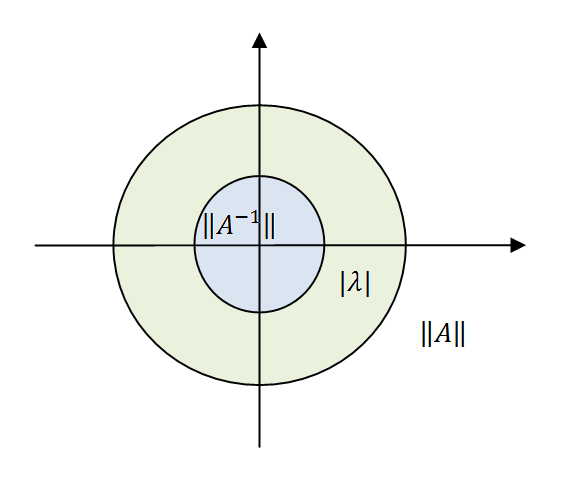
\includegraphics[scale=0.8]{l9_1.png}
\end{center}
\begin{proof}
    Пусть $\lambda$ --- собстенное значение матрицы $A$, то есть, $A\bar x=\lambda\bar x$ для некоторого $\bar x\neq \bar 0$, тогда
    \begin{center}
        $\bar x=\lambda A^{-1} \bar x$\\
        $\lambda^{-1}\bar x=A^{-1}\bar x$
    \end{center}
    То есть, $\lambda^{-1}$ --- собственное значение для матрицы $A^{-1}$.\\
    \begin{center}
        $|\lambda^{-1}|\leqslant||A^{-1}||$ (из оценки)\\~\\
        $|\lambda|^{-1}\leqslant ||A^{-1}||$\\
        $|\lambda|\geqslant \cfrac{1}{||A^{-1}||}$
    \end{center}
    С учетом оценки, получим $$\cfrac{1}{||A^{-1}||}\leqslant|\lambda|\leqslant||A||$$ 
\end{proof}
\begin{definition}
    Матрица называется матрицей \textbf{с диагональным преобладанием}, если каждое из чисел на диагонале больше суммы модулей по строке, то есть, $$\forall i=1,\cdots,n~|a_{ii}|>\sum\limits_{k\neq i}|a_{ik}|.$$
\end{definition} 
\begin{theorem}[1-я Теорема Гершгорина]
    Все собственные значения матрицы $A_{n \times n}=(a_{ij})$ содержатся в объединении кругов на комплексной плоскости. $$|\lambda-a_{ii}|\leqslant \sum\limits_{k=1, k\neq i}^n|a_{ik}|,~i=1,\cdots n.$$
    
    Обозначим: $R_i=\sum\limits_{k=1, k\neq i}^n|a_{ik}|.$
\end{theorem} 
Иными словами, каждое из собственных значений $\lambda$ матрицы $A$ всегда расположено в одном из кругов.
\begin{center}
    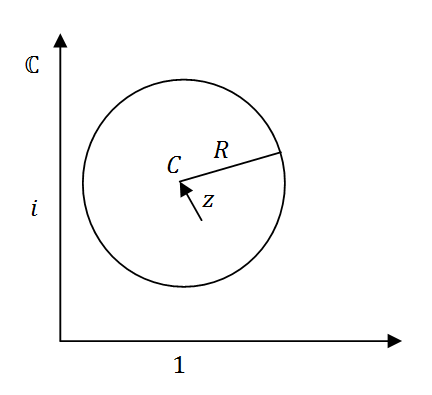
\includegraphics[scale=0.8]{l9_2.png}
\end{center}
$$|z-C|\leqslant R$$
\[\begin{pmatrix}
* & \cdots & \cdots & \cdots & \cdots\\
a_{i1} & \cdots & a_{ii} & \cdots & a_{in}\\
\cdots & \cdots & \cdots & \cdots & *\\
\end{pmatrix}\]
Круг с центром в точке $C=a_{ii}$ и радиусом $R=R_i=\sum\limits_{k\neq i}|a_{ik}|.$\\
\\
Если $\lambda$ --- собственное значение матрицы $A$, то
$$|A-\lambda E|=|(A-\lambda E)^T|=|A^T-\lambda E|=0$$
Получили, что $\lambda$ --- собственное значение матрицы $A^T$.\\ 
У матрицы $A^T$ собственные значения те же, что и у матрицы $A$, а строки $A^T$ --- столбцы $A$. Тогда получаем следствие:
\begin{consequence}
    Все собственные значения матрицы $A$ содержатся в объединении кругов на комплексной плоскости. $$|\lambda-a_{ii}|\leqslant \sum\limits_{k=1, k\neq i}^n|a_{ki}|,~i=1,\cdots n.$$
    
    Обозначим: $C_i=\sum\limits_{k=1, k\neq i}^n|a_{ki}|.$
\end{consequence} 
\begin{proof}
    Пусть $\lambda$ --- собственное значение $A$, докажем, что $\lambda$ находится в объединении кругов Гершгорина.\\
    У каждого собственного значения существует собственный вектор: $$Ax=\lambda x, \bar x\neq \bar 0.$$
    Пусть, например, $|x_1|$ --- наибольший из модулей $|x_i|$, то есть, $|x_1|\geqslant|x_2|,|x_3|,\cdots,|x_n|$. Тогда из $Ax=\lambda x$ следует
    \begin{center}
        $a_{11}x_1+\cdots+a_{1n}x_n=\lambda x_1$\\
        $(\lambda-a_{11})x_1=a_{12}x_2+\cdots+a_{1n}x_n$\\
        $|\lambda-a_{11}||x_1|=|a_{12}|x_2+\cdots+a_{1n}x_n|\leqslant\sum\limits_{k=2}^n|a_{1k}||x_k|\leqslant\sum\limits_{k=2}^n|a_{1k}||x_1|=|x_1|R_1$\\
        $|\lambda-a_{11}|\leqslant R_1=\sum\limits_{k=2}^n|a_{1k}|$
    \end{center}
    Получили, что если $x_1$ --- наибольший, то собственное значение попадает в первый круг Гершгорина. И так далее, если $x_n$ --- наибольший, то собственное значение попадет в $n$-ый круг Гершгорина.
\end{proof}
\begin{consequence}
    Матрица с диагональным преобладанием является невырожденной.
\end{consequence} 
\begin{proof}
    Доказательство следует из того, что в такой матрице все собственные значения $\lambda\neq 0$
\end{proof}
\textbf{Пример 1.}\\
Дана матрица $n\times n$:
\[A=\begin{pmatrix}[r]
2 & -1 & \cdots & \cdots & \cdots & \cdots\\
-1 & 2 & -1 & \cdots & \cdots & \cdots\\
\cdots & -1 & 2 & -1 & \cdots & \cdots\\
\cdots & \cdots & \cdots & \ddots & \cdots & \cdots\\
\cdots & \cdots & \cdots & -1 & 2 & -1\\
\cdots & \cdots & \cdots & \cdots & -1 & 2\\
\end{pmatrix}\]
Вычислим круги Гершгорина.
\begin{center}
    \begin{tabular}{|c|c|c|}
        \hline
        № & Центр & Радиус \\ \hline
        1 & 2 & |-1|=1 \\ \hline
        2~--~(n-1) & 2 & |-1|+|-1|=2 \\ \hline
        n & 2 & |-1|=1 \\ \hline
    \end{tabular}\\
    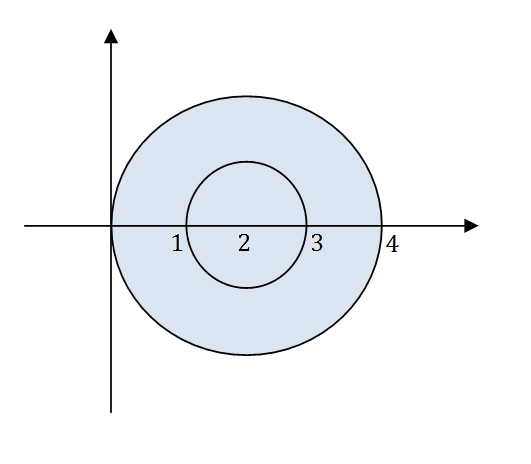
\includegraphics[scale=0.8]{l9_3.png}
\end{center}
Все собственные значения содержатся в объединении кругов на комплексной плоскости.\\
\begin{center}
    $|\lambda-2|\leqslant 1$\\
    $|\lambda-2|\leqslant 2$
\end{center}
$
\left\{
\begin{array}{lcl}
A^*=A \\
A\in M_n(\mathbb{R}) \\
\end{array}
\right.
$\\ \\
Получили, что $\lambda_i\in \mathbb{R},~0\leqslant\lambda_i\leqslant 4$.

\subsection{Кратности собственных значений}
\begin{definition}
    Если $\chi_A(\lambda)=(\lambda_1-\lambda)^{k_1}\cdots(\lambda_s-\lambda)^{k_s}$, где $\lambda_i$ различны, то числа $k_i$ называют \textbf{кратностями} соответствующих собственных значений.
\end{definition}
\begin{theorem}[2-я Теорема Гершгорина] Если объединение $U$ $r$ кругов Гершгорина не пересекается с остальными $(n-r)$ кругами, то $U$ содержит ровно $r$ собственных значений с учетом кратностей.
\end{theorem}
\begin{proof}
Пусть $D$ --- диагональная часть матрицы $A$
\[D=\begin{pmatrix}
a_{11} & \cdots & 0 \\
\vdots & \ddots & \vdots \\
0 & \cdots & a_{nn} \\
\end{pmatrix}\]
а матрица $B=A-D$ --- матрица $A$ без диагональных элементов 
\[B=\begin{pmatrix}
0 & a_{12} & \cdots \\
a_{21} & \ddots & \cdots \\
\cdots & \cdots & 0 \\
\end{pmatrix}\]
Рассмотрим непрерывное непрерывное семейство матриц $$A_t=D+tB$$
Это непрерывная функция из $\mathbb{R}$ в $M_n(\mathbb{C})$. Здесь $A_0=D,~A_1=A$.\\
Корни характеристического многочлена матрицы $A_t$ непрерывно зависят от $t_0$. При $t=0$ --- это $\lambda_1(0)=a_{11},\cdots,\lambda_n(0)=a_{nn}$, а при $t=1$ --- это собственные числа матрицы $A$.\\
По первой теореме Гершгорина $\forall t~\lambda\in U$ в объединении кругов Гершгорина с центрами $a_{11},\cdots,a_{nn}$ и радиусами $$R_i(t)=tR_i.$$
С ростом $t$ круги "раздуваются" из точек (движение по непрервной кривой).
\begin{center}
    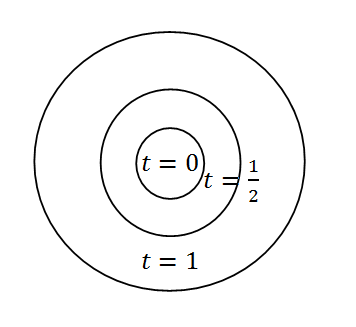
\includegraphics[scale=0.8]{l9_4.png}
\end{center}
Если объединение некоторых $r$ кругов Гершгорина не пересекаются с остальными при $t=1$, то и при $t<1$ тоже, значит каждое из соответствующих $r$ собственных значений $\lambda_i$ двигается из $a_{ii}$ по непрерывной кривой внутри $U.$
\end{proof}
\textbf{Пример 2.}\\
Пусть 
\[A=\begin{pmatrix}[r]
-1 & 1 \\
-4 & -5 \\
\end{pmatrix}\]
\[\chi_A(\lambda)=|A-\lambda E|=\begin{vmatrix}[r]
-1-\lambda & 1 \\
-4 & -5-\lambda \\
\end{vmatrix}=(\lambda +3)^2\]
Получили, что $\lambda_1=\lambda_2=-3$.
\begin{center}
    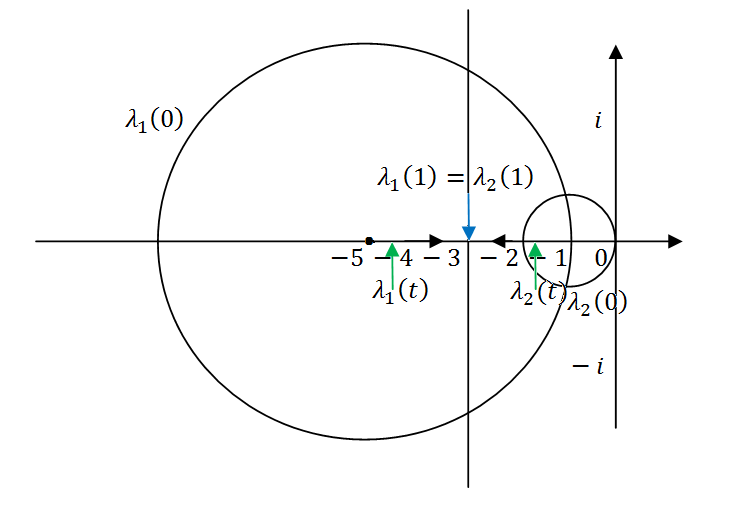
\includegraphics[scale=0.8]{l9_5.png}
\end{center}
\[A=\begin{pmatrix}[r]
-1 & t \\
-4t & -5 \\
\end{pmatrix}=\begin{pmatrix}[r]
-1 & 0 \\
0 & -5 \\
\end{pmatrix}+ t\begin{pmatrix}[r]
0 & 1 \\
-4 & 0 \\
\end{pmatrix}\]
Характеристический многочлен $$\chi_{A_t}(\lambda)=|A_t-\lambda E|=\lambda^2+6\lambda+5+4t^2$$
\begin{center}
    $\lambda_{1,2}=-3\pm 2\sqrt{1-t^2},~t<1$\\
    $\lambda_{1,2}=-3\pm i\cdot 2\sqrt{1-t^2},~t>1$
\end{center}
\textbf{Пример 3.}\\
\[A=\begin{pmatrix}
5 & 1 & 0 \\
0 & 1 & 2 \\
0 & 2 & 1 \\
\end{pmatrix}\]
Для матрицы $A$:
\begin{center}
    $|\lambda-5|\leqslant 1$\\
    $|\lambda-1|\leqslant 2$ --- 2 раза
\end{center}
\begin{center}
    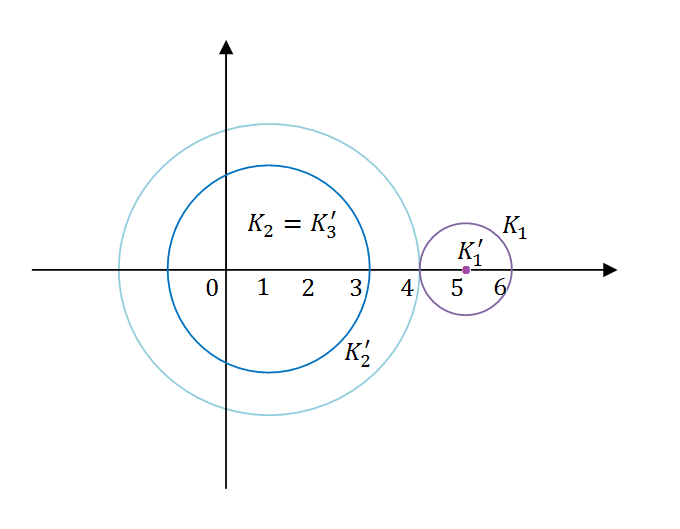
\includegraphics[scale=0.8]{l9_6.png}
\end{center}
В $K_1$ находится одно собственное значение $\lambda_1$, в $K_2$ --- два $\lambda_2,~\lambda_3$.\\
Для матрицы $A^T$
\[A^T=\begin{pmatrix}
5 & 0 & 0 \\
1 & 1 & 2 \\
0 & 2 & 1 \\
\end{pmatrix}\]
\begin{center}
    $K_1':~|\lambda-5|=0 \Rightarrow \lambda_1'=5$\\
    $K_2':~|\lambda-1|\leqslant 3$\\
    $K_3':~|\lambda-1|\leqslant 2$
\end{center}
То есть, $\lambda_2',~\lambda_3'\in K_2'=K_2'\cup K_3'$.\\
Так как $\{\lambda_1,~\lambda_2,~\lambda_3\}=\{\lambda_1',~\lambda_2',~\lambda_3'\}$ --- те же собственные значения, то $\lambda_1=\lambda_1=5$.\\
Значит $\lambda_2'$ и $\lambda_3'$ --- те же, что $\lambda_2$ и $\lambda_3$, то есть, $\lambda_2',~\lambda_3'\in K_2$.\\
Итог для матрицы $A$: $\lambda_1=5$, а $\lambda_2,~\lambda_3$ удовлетворяют условию $|\lambda-1|\leqslant 2$.
\subsection{Домашнее задание 9}\begin{enumerate}
    \item Нарисовать круги Гершгорина для матрицы $A$ и с их помощью оценить собственные значения. Вычислить собственные значения и сравнить результаты.
    \[A = \begin{pmatrix}
    5 & 0.3\\
    -0.5 & 2\\
    \end{pmatrix}\]
    \item С помощью теоремы Гершгорина нарисовать область, где находятся собственные значения матрицы $A$.
    \[A = \begin{pmatrix}
    3 & 0.2 & -0.2\\
    0 & 2 & 0.1\\
    0.1 & 0.4 & 1\\
    \end{pmatrix}\]
    \item Доказать, что определитель матрицы $A$ не равен 0 ($detA\neq 0$). Нарисовать наименьшую область, содержащую собственные значения.
    \[A = \begin{pmatrix}
    2 & cos~x & cos^2~x\\
    0 & 5 & sin^2~x\\
    3sin^2~x & 3 & 10\\
    \end{pmatrix}\]
    \item Доказать, что в номерах 1, 2 и 3 все собственные значения --- положительные действительные числа и оценить их.\\
    Подсказка: если $\lambda$ --- собственное значение матрицы $A$, то и $\overline \lambda$ --- тоже ее собственное значение, так как $|\overline{A-\lambda E}|=|A-\overline\lambda E|=0$.
\end{enumerate}
